%  DOCUMENT CLASS
\documentclass[11pt]{article}

%PACKAGES
\usepackage[utf8]{inputenc}
%\usepackage[ngerman]{babel}
\usepackage[reqno,fleqn]{amsmath}
\setlength\mathindent{10mm}
\usepackage{amssymb}
\usepackage{amsthm}
\usepackage{color}
\usepackage{delarray}
% \usepackage{fancyhdr}
\usepackage{units}
\usepackage{times, eurosym}
\usepackage{verbatim} %Für Verwendung von multiline Comments mittels \begin{comment}...\end{comment}
\usepackage{wasysym} % Für Smileys
\usepackage{gensymb} % Für \degree
\usepackage{graphicx}
\usepackage{tikz}
\usepackage{mathtools}
\usepackage{stmaryrd}

% FORMATIERUNG
\usepackage[paper=a4paper,left=25mm,right=25mm,top=25mm,bottom=25mm]{geometry}
\usepackage{array}
\usepackage{fancybox} %zum Einrahmen von Formeln
\setlength{\parindent}{0cm}
\setlength{\parskip}{1mm plus1mm minus1mm}

\allowdisplaybreaks[1]


% PAGESTYLE

%MATH SHORTCUTS
\newcommand{\NN}{\mathbb N}
\newcommand{\ZZ}{\mathbb Z}
\newcommand{\QQ}{\mathbb Q}
\newcommand{\RR}{\mathbb R}
\newcommand{\CC}{\mathbb C}
\newcommand{\KK}{\mathbb K}
\newcommand{\U}{\mathbb O}
\newcommand{\eqx}{\overset{!}{=}}
\newcommand{\Det}{\mathrm{Det}}
\newcommand{\Gl}{\mathrm{Gl}}
\newcommand{\diag}{\mathrm{diag}}
\newcommand{\sign}{\mathrm{sign}}
\newcommand{\rang}{\mathrm{rang}}
\newcommand{\cond}{\mathrm{cond}_{\| \cdot \|}}
\newcommand{\conda}{\mathrm{cond}_{\| \cdot \|_1}}
\newcommand{\condb}{\mathrm{cond}_{\| \cdot \|_2}}
\newcommand{\condi}{\mathrm{cond}_{\| \cdot \|_\infty}}
\newcommand{\eps}{\epsilon}

\setlength{\extrarowheight}{1ex}

\begin{document}
	
	\begin{center}
		\textbf{
			Exercises: Introduction to Robotics, SS 2016\\
			Assignment \#6\\
		}
		
		\begin{tabular}{lll}
			& \\
			by & Jonas Papmeier & Mat Nr. 6326394\\
			& Jan Fabian Schmid & Mat.Nr. 6440383\\
			\\
			\hline
		\end{tabular}
	\end{center}
	
	\subsection*{Task 6.1.1}

Task 6.1.1 is directly merged with 6.1.2 due to similarity.

\subsection*{Task 6.1.2}

Figure \ref{fig:wspace} displays the workspace with the two circular obstacles and the start and goal positions. No paths were calculated from start to goal positions.
Similar Figure \ref{fig:cspace} displays the configuration space with the same objects in the surrounding
\begin{figure}[h]
	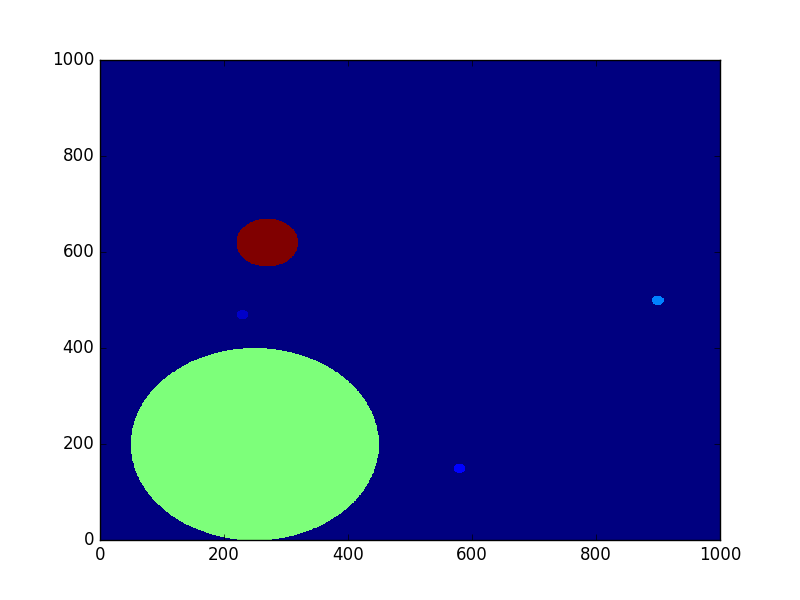
\includegraphics[width=0.9\textwidth ,height=0.94\textwidth]{Wspace.png}
	\caption{Workspace of the robot, red: obstacle 1 ;light green: obstacle 2; light blue: start position; blue: goal position; dark blue: background/free space}
	\label{fig:wspace}
\end{figure}

\begin{figure}[h]
	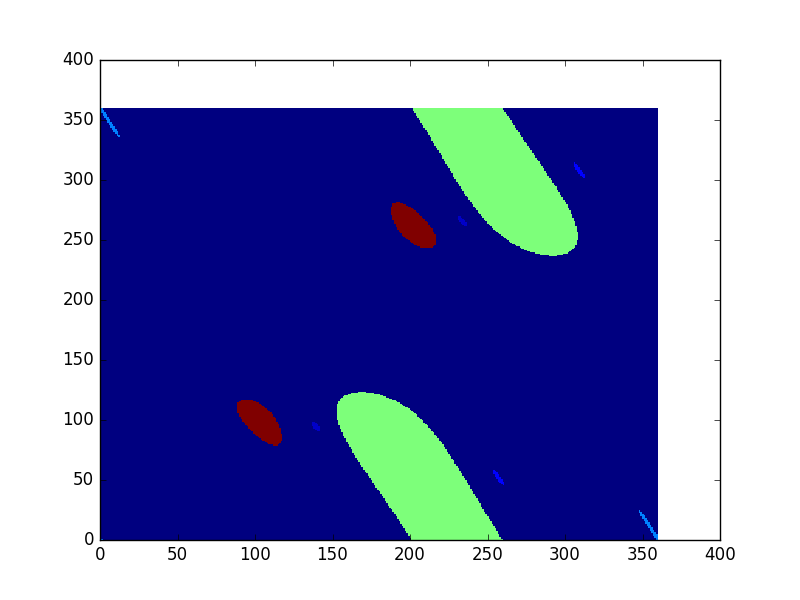
\includegraphics[scale=0.7]{Cspace.png}
	\caption{Configuration space of the robot, red: obstacle 1 ;light green: obstacle 2; light blue: start position; blue: goal position; dark blue: background/free space}
	\label{fig:cspace}
\end{figure}



	
\end{document}
